\documentclass{beamer}
\usepackage{CJKutf8}
\usepackage{amsfonts}
\usepackage{amsmath}
\usepackage{amssymb}
\usepackage{amsthm}
\usepackage{enumerate}
\usepackage{graphicx}
\usepackage{layout}
\usepackage{mathrsfs}
\usepackage{fancyhdr}
\usepackage{subfigure}
\usepackage{tcolorbox}
\usepackage{tikz-cd}
\usepackage{color}
\usepackage{pifont}
\usepackage{verbatim}

\usepackage{mathtools}
\usepackage{float}
\usepackage{bm}
\usetheme{AnnArbor}
% \usetheme{Antibes}
\usecolortheme{beaver}

\setbeamertemplate{navigation symbols}{}
\newcommand{\dif}{\mathrm{d}}
\newtheorem{thm}{{定理}}
\begin{document}

\begin{CJK*}{UTF8}{gkai}
  \title{中期考核答辩}
  \author{李阳\, \\
    专业: 计算数学\, 导师: 张庆海}
  \date{2021年11月3日}
  \maketitle

  \begin{frame}
    \frametitle{目录}
    \tableofcontents
  \end{frame}

  \section{课程学习}

  \begin{frame}
    \frametitle{课程成绩}
    \begin{columns}
      \begin{column}{.5\linewidth}
        \begin{itemize}
        \item
          微分方程数值解: \textcolor{red}{100};
        \item
          计算科学前沿问题选讲: \textcolor{red}{100};
        \item
          偏微分方程: 87;
        \item
          非线性问题的数学方法: 88;
        \item
          代数拓扑: 86;
        \item
          泛函分析: 82;
        \item
          ...
        \end{itemize}
      \end{column}
      \begin{column}{.5\linewidth}
        \begin{itemize}
        \item
          英语六级成绩: \textcolor{red}{623}
        \end{itemize}
        \begin{center}
          
\includegraphics[scale=0.30]{./png/cet6}
        \end{center}
      \end{column}
    \end{columns}
  \end{frame}

  \section{研究内容}
  \begin{frame}
    \frametitle{研究内容: 不可压\,Navier-Stokes\,方程的高阶数值方法}
    \begin{itemize}
    \item 无滑移边界下不可压\,Navier-Stokes\,方程的无量纲形式:
      \begin{equation}
        \label{eq:INSE}
        \begin{split}
          \frac{\partial \bm{u}}{\partial t}+ \left( \bm{u}\cdot\nabla \right)\bm{u} &= \bm{g}-\nabla p+\nu\Delta \bm{u} \text{ in } \Omega_T, \\
          \nabla\cdot \bm{u} &= 0 \hspace{23mm} \text{ in } \Omega_T, \\
          \bm{u} &= \mathbf{0} \hspace{23mm} \text{ on } \partial\Omega_T,
        \end{split}
      \end{equation}
      其中\,$\Omega_T=\Omega\times (0, T], \,\partial\Omega_T=\partial\Omega\times (0, T]$.

%    \item
%      三维空间中不可压\,Navier-Stokes\,方程全局解的存在性与正则性是\textcolor{red}{千禧年七大数学难题}之一.
      
    \item
%      (\ref{eq:INSE})\,式作为流体力学的基本控制方程,
%      不可压\,Navier-Stokes\,方程
      (\ref{eq:INSE})\,式描述了粘性不可压缩流体(如海洋流动)的\textcolor{red}{普遍}运动规律,
      对其进行高精度数值模拟对于科学研究和工程应用具有重大意义.
    \end{itemize}
  \end{frame}

  \section{前期准备}
  \begin{frame}
    \frametitle{前期准备\ding{172}: 物理 $\rightarrow$ 数学}
    \begin{itemize}
    \item
      由\textcolor{red}{质量}, \textcolor{red}{动量}, \textcolor{red}{能量守恒定律}出发
      严格推导不可压\,Navier-Stokes\,方程.
      \begin{align*}
        \left( \bm{u}\cdot\nabla \right)\bm{u} &\Leftrightarrow \text{对流项}, \\
        \Delta \bm{u} &\Leftrightarrow \text{扩散项}, \\
        \nabla\cdot \bm{u}=0 &\Leftrightarrow \text{不可压条件}.
      \end{align*}
    \item
      \textcolor{red}{Helmholtz\,分解定理}:
      \begin{equation*}
        \bm{u}^{*} = \mathscr{P}\bm{u}^{*}+\nabla\phi,
      \end{equation*}
      其中
      \begin{equation*}
        \nabla\cdot \mathscr{P}\bm{u}^{*}=0 \text{ in } \Omega, \qquad
        \bm{n}\cdot \mathscr{P}\bm{u}^{*} = 0 \text{ on } \partial\Omega.
      \end{equation*}
    \item ...
    \end{itemize}
  \end{frame}

  \begin{frame}
    \begin{itemize}
    \item
      将所学内容整理为讲义,
      \textcolor{red}{构建知识体系}.
    \end{itemize}
    \begin{columns}
      \begin{column}{.5\linewidth}
        \begin{center}
          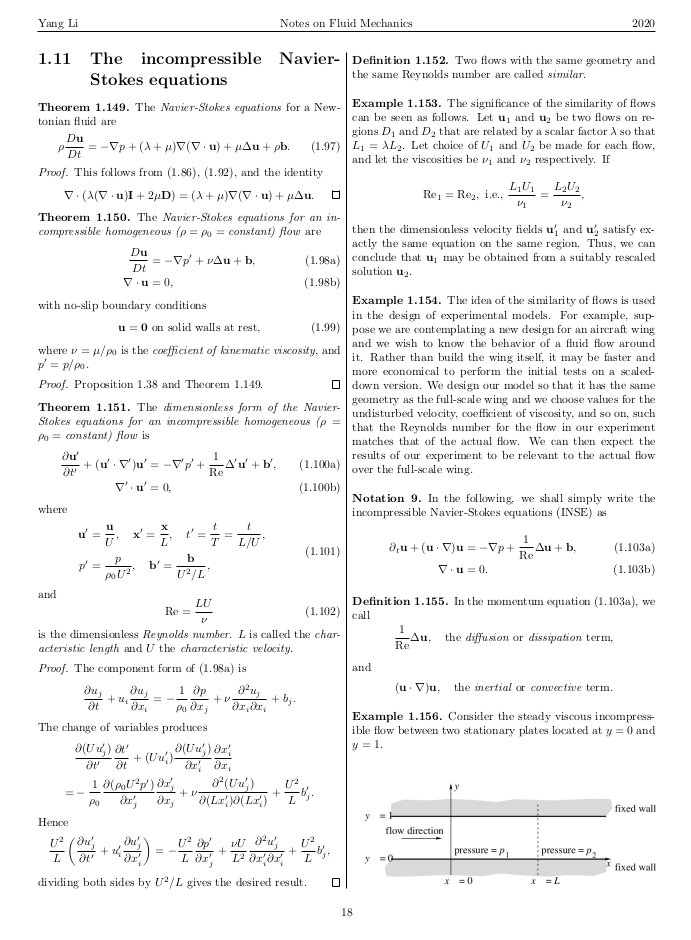
\includegraphics[scale=0.22]{./png/fmnotes}
        \end{center}
      \end{column}
      \begin{column}{.5\linewidth}
        \begin{center}
          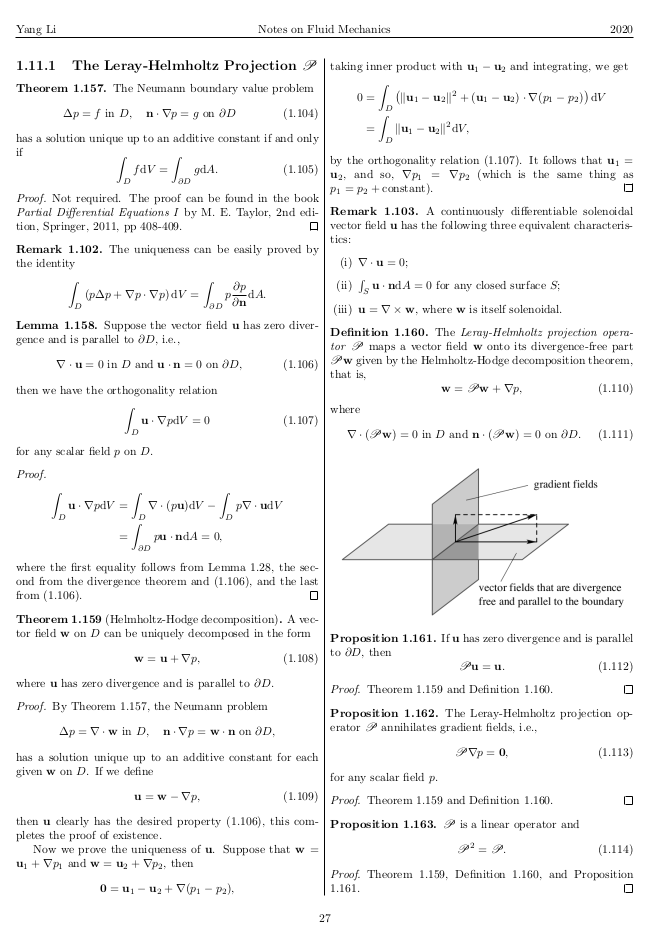
\includegraphics[scale=0.22]{./png/helmholtz}
        \end{center}
      \end{column}
    \end{columns}
  \end{frame}
  
  \begin{frame}
    \frametitle{前期准备\ding{173}: 数学 $\rightarrow$ 数值方法}
    \begin{itemize}
    \item
      阅读相关经典文献, 撰写文献综述.
    \end{itemize}
    \begin{center}
      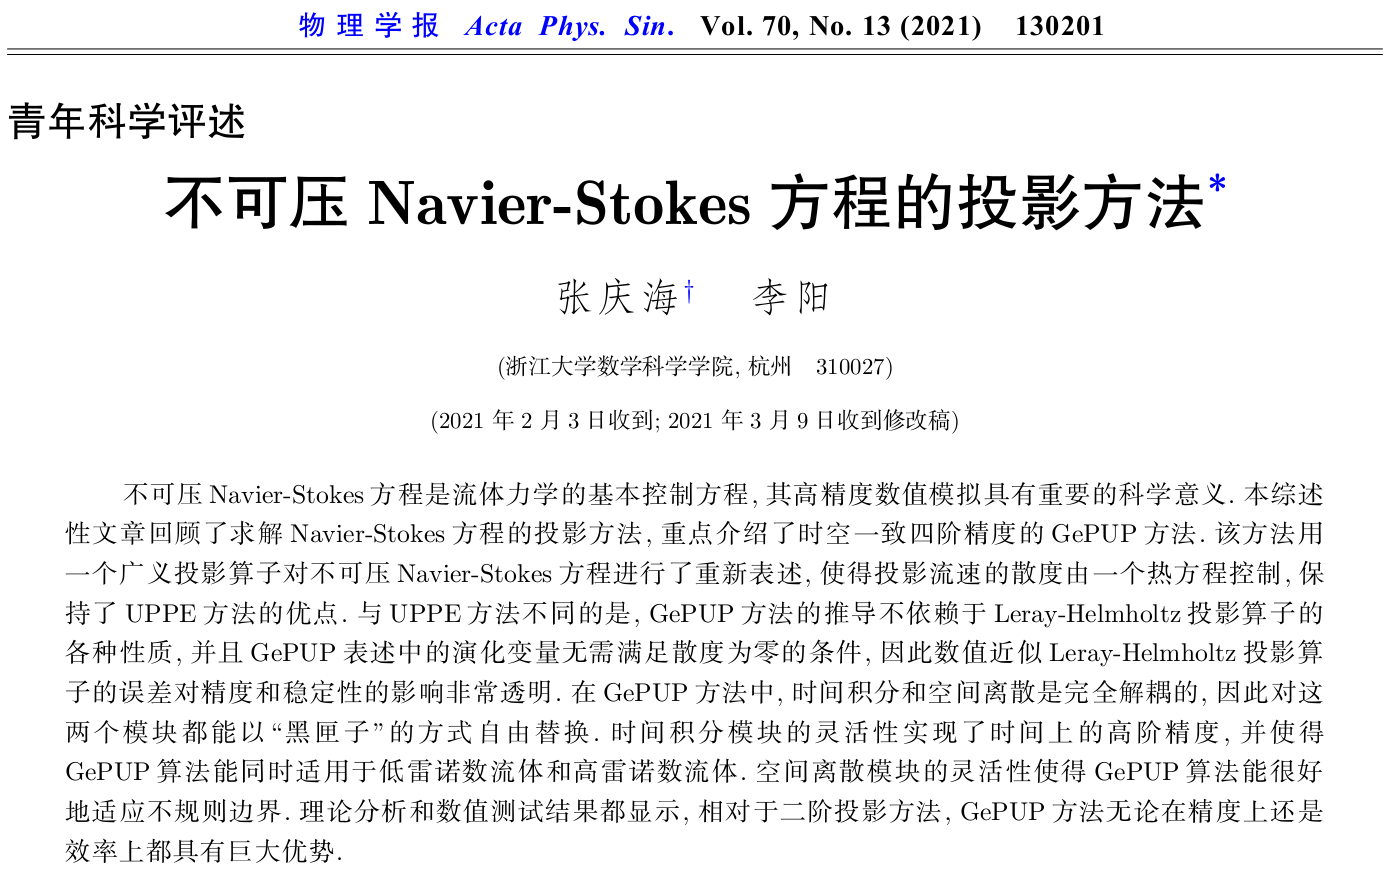
\includegraphics[scale=0.22]{./png/methods}
    \end{center}
  \end{frame}

  \begin{frame}
    \begin{itemize}
    \item
      数值求解不可压\,Navier-Stokes\,方程的主要困难:
      如何\textcolor{red}{高效}地处理不可压约束条件\,$\nabla\cdot \bm{u}=0$?
    \item
      一阶\textcolor{red}{投影方法}:
      \begin{align*}
        \frac{\bm{u}^{*}-\bm{u}^n}{\delta t} &= -\bm{C}\left( \bm{u}^{*}, \bm{u}^n \right) + \bm{g}^n+\nu \Delta \bm{u}^{*}, \\
        \bm{u}^{n+1} &= \bm{P}\bm{u}^{*},
      \end{align*}
      其中\,$\bm{P}\approx \mathscr{P}$.

      \textcolor{red}{优势}:
      \begin{itemize}
      \item \textcolor{red}{效率高}:
        流速和压强在计算域内解耦,
        每个时间步仅需求解若干个关于压强或流速的椭圆边值问题;
      \item
        可推广到\textcolor{red}{二阶精度}.
      \end{itemize}
      \textcolor{red}{劣势}:
      \begin{itemize}
      \item
        辅助变量\,$\bm{u}^{*}$\,不具有物理意义,
        其边界条件依赖于具体时间积分方法的细节;
      \item
        无法直接将求解常微分方程组的高阶方法作为``黑匣子''使用.
      \end{itemize}
    \end{itemize}
  \end{frame}

  \begin{frame}
    \textcolor{red}{GePUP\,表述}:
    \begin{subequations}
      \label{eq:GePUP}
      \begin{align}
        \frac{\partial\bm{w}}{\partial t}
        &= \bm{g} -\left(\bm{u}\cdot\nabla\right)\bm{u}
          -\nabla q
          + \nu\Delta\bm{w}
          \qquad \textrm{in }\  \Omega_T,
        \\
        \bm{w} & = \bm{0}
                 \hspace{51mm} \textrm{on }\ \partial \Omega_T,
        \\
        \bm{u} &= \mathscr{P} \bm{w}
                 \hspace{46mm} \textrm{in }\  \Omega_T,
        \\
        \bm{u}\cdot \bm{n} & = 0 
                             \hspace{51mm} \textrm{on }\ \partial \Omega_T,
        \\
        \Delta q &= \nabla\cdot \left(
                   \bm{g} -\left(\bm{u}\cdot\nabla\right)\bm{u}
                   \right)
                   \hspace{22mm} \textrm{in }\  \Omega_T,
        \\
        \bm{n}\cdot\nabla q
        &= \bm{n}\cdot \left(
          \bm{g} + \nu\Delta\bm{u}-\nu\nabla\nabla\cdot\bm{u}
          \right) \hspace{11mm} \textrm{on }\ \partial \Omega_T.
      \end{align}
    \end{subequations}
    基于该表述构造数值方法具有如下优势:
    \begin{itemize}
    \item
      \textcolor{red}{时空一致四阶精度};
    \item
      \textcolor{red}{最优求解复杂度}:
      单个时间步为\,$O(N)$,
      其中\,$N$\,是控制体数目;
    \item
      \textcolor{red}{时间积分与空间离散完全解耦};
    \item
      $\bm{w}$\,的散度由一个\textcolor{red}{热方程}控制:
      \begin{equation*}
        \frac{\partial \left( \nabla\cdot\bm{w} \right)}{\partial t} = \nu\Delta \left( \nabla\cdot \bm{w} \right).
      \end{equation*}
    \end{itemize}
  \end{frame}

  \begin{frame}
    \frametitle{前期准备\ding{174}: 数值方法 $\rightarrow$ 计算机编程实现}
    \begin{itemize}
    \item
      系统学习\,C++\,编程语言;
    \item
      熟悉\,Linux\,操作系统下的常用工具,
      如\,emacs, auctex, make, git\,等;
    \item
      基本\,C++\,编程训练:
      \begin{itemize}
      \item
        多重网格方法的程序设计;
      \item
        平面上具有任意复杂拓扑结构集合的高效表示及布尔代数运算.
        % \begin{figure}[h]
        %   \centering
        %   \subfigure{
        %   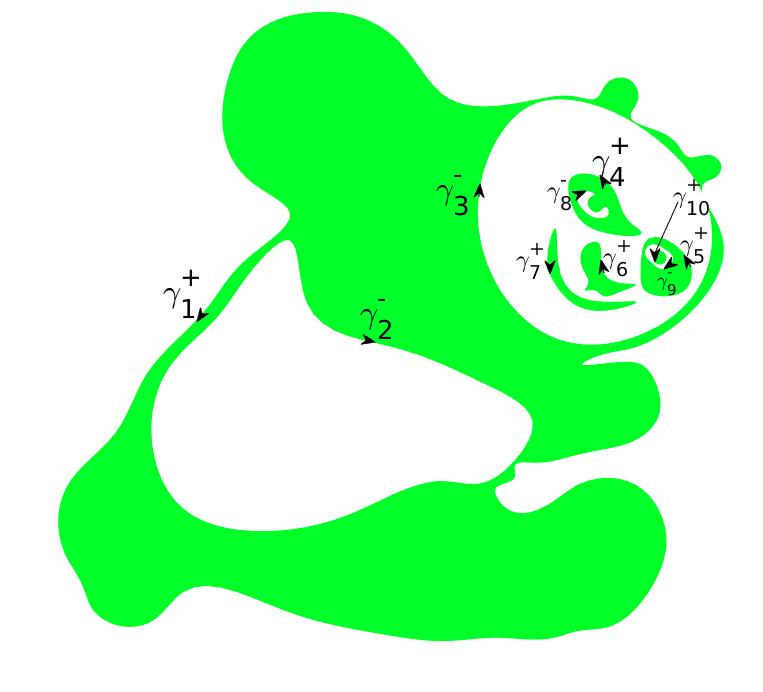
\includegraphics[width=0.42\linewidth]{./png/pandaHasse}
        % }
        %   \hfill
        %   \subfigure{
        %   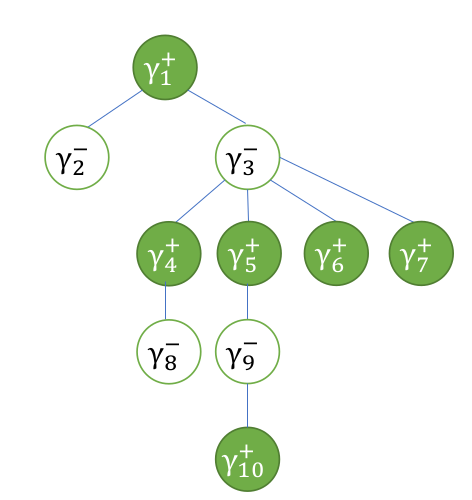
\includegraphics[width=0.42\linewidth]{./png/pandaHasse2}
        % }
        %   \caption{熊猫的高效表示}
        % \end{figure}
      \end{itemize}
    \end{itemize}
    \begin{center}
      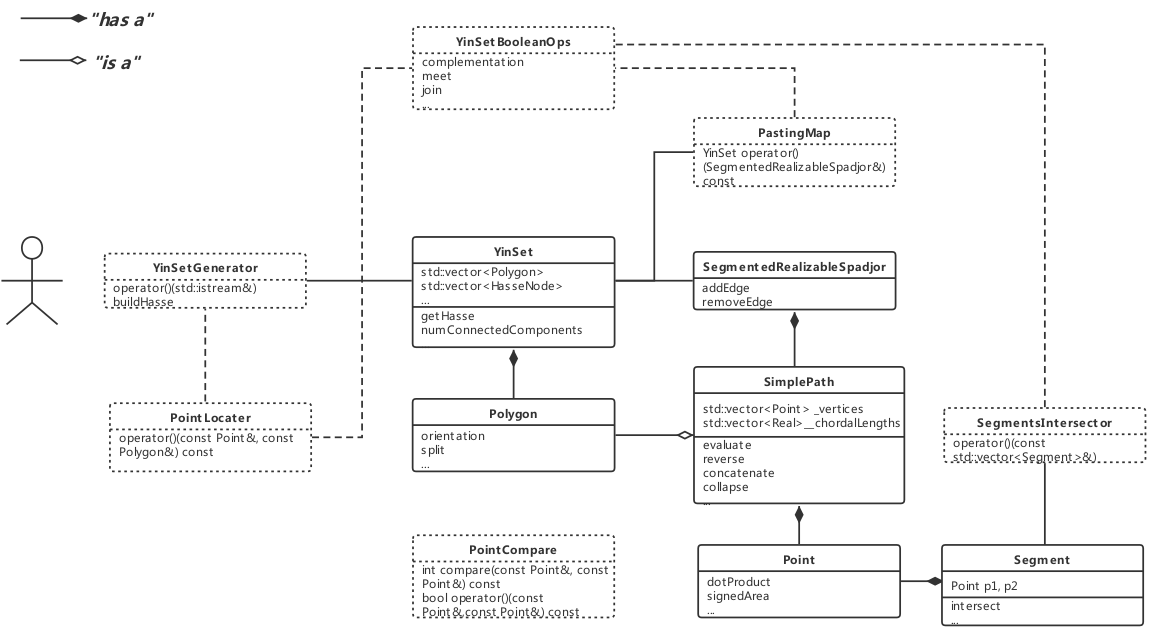
\includegraphics[scale=0.24]{./png/uml}
    \end{center}
  \end{frame}
  
  \section{研究进展}
  \begin{frame}
    \frametitle{研究进展: 求解不可压\,Navier-Stokes\,方程的能量稳定算法}
    \begin{thm}[不可压\,Navier-Stokes\,方程的能量耗散性质]
      考虑粘性不可压流体且外力为保守力的情况下,
      以下动能耗散式成立:
      \begin{equation}
        \frac{\dif}{\dif t}E_{\text{kinetic}} = -\nu\int_{\Omega}\left\|  \nabla \bm{u}\right\|^2\dif \bm{x} \le 0,
      \end{equation}
      其中
      \begin{equation}
        E_{\text{kinetic}} := \frac{1}{2}\int_{\Omega} \left\|  \bm{u}\right\|^2\dif \bm{x}.
      \end{equation}
    \end{thm}

    \begin{itemize}
    \item \textcolor{red}{目标}:
      设计具有类似能量耗散性质的数值方法.
    \end{itemize}
  \end{frame}

  \begin{frame}
    \frametitle{GePUP-SAV\,能量稳定算法}
    引入标量辅助变量\,$r(t)\equiv 1$\,满足
    \begin{equation}
      \frac{\dif r}{\dif t} = 0 = \int_{\Omega} \left( \left( \bm{u}\cdot\nabla \right)\bm{u} \right)\cdot \bm{u}\, \dif \bm{x},
    \end{equation}
    将\,GePUP\,表述等价地写为
    \begin{subequations}
      \label{eq:GePUP}
      \begin{align}
        \frac{\partial\bm{w}}{\partial t}
        &= \bm{g} -r(t)\left(\bm{u}\cdot\nabla\right)\bm{u}
          -\nabla q
          + \nu\Delta\bm{w}
          \qquad \textrm{in }\  \Omega_T,
        \\
        \bm{w} & = \bm{0}
                 \hspace{58mm} \textrm{on }\ \partial \Omega_T,
        \\
        \frac{\dif r}{\dif t} &= \int_{\Omega} \left( \left( \bm{u}\cdot\nabla \right)\bm{u} \right)\cdot \bm{u}\, \dif \bm{x},
        \\
        \bm{u} &= \mathscr{P} \bm{w}
                 \hspace{52mm} \textrm{in }\  \Omega_T,
        \\
        \bm{u}\cdot \bm{n} & = 0 
                             \hspace{57mm} \textrm{on }\ \partial \Omega_T,
        \\
        \Delta q &= \nabla\cdot \left(
                   \bm{g} -r(t)\left(\bm{u}\cdot\nabla\right)\bm{u}
                   \right)
                   \hspace{21mm} \textrm{in }\  \Omega_T,
        \\
        \bm{n}\cdot\nabla q
        &= \bm{n}\cdot \left(
          \bm{g} + \nu\Delta\bm{u}-\nu\nabla\nabla\cdot\bm{u}
          \right) \hspace{17mm} \textrm{on }\ \partial \Omega_T.
      \end{align}
    \end{subequations}
    
  \end{frame}

  \begin{frame}
    应用\,Crank-Nicolson\,方法作时间离散得以下\,\textcolor{red}{GePUP-SAV-CN\,半离散格式}:
    \begin{align*}
      \frac{\bm{w}^{n+1}-\bm{w}^n}{\delta t} &= \bm{g}^{n+\frac{1}{2}}-r^{n+\frac{1}{2}}\widetilde{\bm{u}}^{n+1/2}\cdot\nabla \widetilde{\bm{u}}^{n+1/2}-\nabla q^{n+1/2}+\nu\Delta \bm{w}^{n+\frac{1}{2}} \text{ in } \Omega, \\
      \bm{w}^{n+1} &= \bm{0} \hspace{84mm}\text{ on } \partial\Omega, \\
      \frac{r^{n+1}-r^n}{\delta t} &= \int_{\Omega}(\widetilde{\bm{u}}^{n+1/2}\cdot\nabla \widetilde{\bm{u}}^{n+1/2})\cdot \bm{u}^{n+\frac{1}{2}}\dif \bm{x}, \\
      \bm{u}^{n+1} &= \mathscr{P}\bm{w}^{n+1} \hspace{74mm}\text{ in } \Omega, \\
      \bm{u}^{n+1}\cdot \bm{n} &= 0 \hspace{84mm}\text{ on } \partial\Omega, \\
      \Delta q^{n+1/2} &= \nabla\cdot \left(\bm{g}^{n+\frac{1}{2}}-r^{n+\frac{1}{2}}\widetilde{\bm{u}}^{n+1/2}\cdot\nabla \widetilde{\bm{u}}^{n+1/2}\right) \hspace{27mm}\text{ in } \Omega, \\
      \bm{n}\cdot \nabla q^{n+1/2} &= \bm{n}\cdot\left(\bm{g}^{n+\frac{1}{2}}+\nu\Delta \widetilde{\bm{u}}^{n+1/2}-\nu\nabla\nabla\cdot \widetilde{\bm{u}}^{n+1/2}\right) \hspace{19mm}\text{ on } \partial\Omega,
    \end{align*}
    其中上标\,$^{n+\frac{1}{2}}$\,表示时间步\,$n$\,和\,$n+1$\,的平均值,
    $\widetilde{\bm{u}}^{n+1/2}$\,由外插公式得到.

    \begin{itemize}
    \item
      对\,$\bm{w}^{n+1}$, $\bm{u}^{n+1}$, 和\,$q^{n+1/2}$\,作分解后,
      可实现对上述格式的高效求解.
    \end{itemize}
  \end{frame}

  \begin{frame}
    \begin{thm}[GePUP-SAV-CN\,半离散格式的\textcolor{red}{修正}能量耗散性质]
      \begin{equation}
        \frac{1}{\delta t}\left( \mathcal{E}\left( t^{n+1} \right)-\mathcal{E}\left( t^n \right) \right) \le -\nu\int_{\Omega}\left\|\nabla\bm{u}^{n+\frac{1}{2}}\right\|^2\dif \bm{x}
      \end{equation}
      其中
      \begin{equation}
        \mathcal{E}\left( t^n \right) := \frac{1}{2}\int_{\Omega}\left\|\bm{u}^n\right\|^2\dif \bm{x}+\frac{1}{2}\left|r^n\right|^2.
      \end{equation}
    \end{thm}

    \begin{itemize}
    \item 时间离散方法选为向后微分公式\,(BDF)\,或\,
      Gauss-Legendre Runge-Kutta\,方法,
      仍有类似离散能量耗散结论成立.
    \end{itemize}
  \end{frame}
  \section{后期研究计划}
  \begin{frame}
    \frametitle{后期研究计划}
    % \textcolor{red}{总结}:
    % \begin{itemize}
    % \item
    %   夯实基础,
    %   构建知识体系:
    %   微分方程数值解, 流体力学;
    % \item

    % \end{itemize}

    \begin{itemize}
    \item
      在现有\,C++\,程序框架下实现\,GePUP-SAV\,能量稳定算法.
    \end{itemize}
  \end{frame}

  \section*{}
  \begin{frame}
    \centering\huge
    \textcolor{red}{敬请各位老师批评指正!}
  \end{frame}

\end{CJK*}

\end{document}
%%% Local Variables:
%%% mode: latex
%%% TeX-master: t
%%% End:
